\documentclass[11pt]{beamer}
\usetheme{Warsaw}
\usepackage[utf8]{inputenc}
\usepackage[english]{babel}
\usepackage{amsmath}
\usepackage{amsfonts}
\usepackage{amssymb}
\usepackage{graphicx}
\author{Tim Reiprich, Tegshigzugder Otgonbayar, Luca Maltagliati}
\title{IoT Project: Height / Capacity Monitor}
%\setbeamercovered{transparent} 
%\setbeamertemplate{navigation symbols}{} 
%\logo{} 
%\institute{} 
%\date{} 
%\subject{} 
\begin{document}

\begin{frame}
\titlepage
\end{frame}

%\begin{frame}
%\tableofcontents
%\end{frame}

%functionality
%actions to save energy and make the system robust
%explain and show general implementation
%What doesn't work and possible problems
%questions

\begin{frame}{Overview}
\begin{itemize}
\item design of a system to check level of fluid in a basket
\item measure height using an ultrasonic sensor and send it to central computer
\item show if certain thresholds (low/high) are surpassed at basket and central computer using LEDs and Node-Red
\item thresholds can be dynamically set using the Node-Red interface and are sent to the ESP connected to the sensor
\end{itemize}
\end{frame}

\begin{frame}{Circuit}
\begin{figure}
\hspace*{-0.5cm}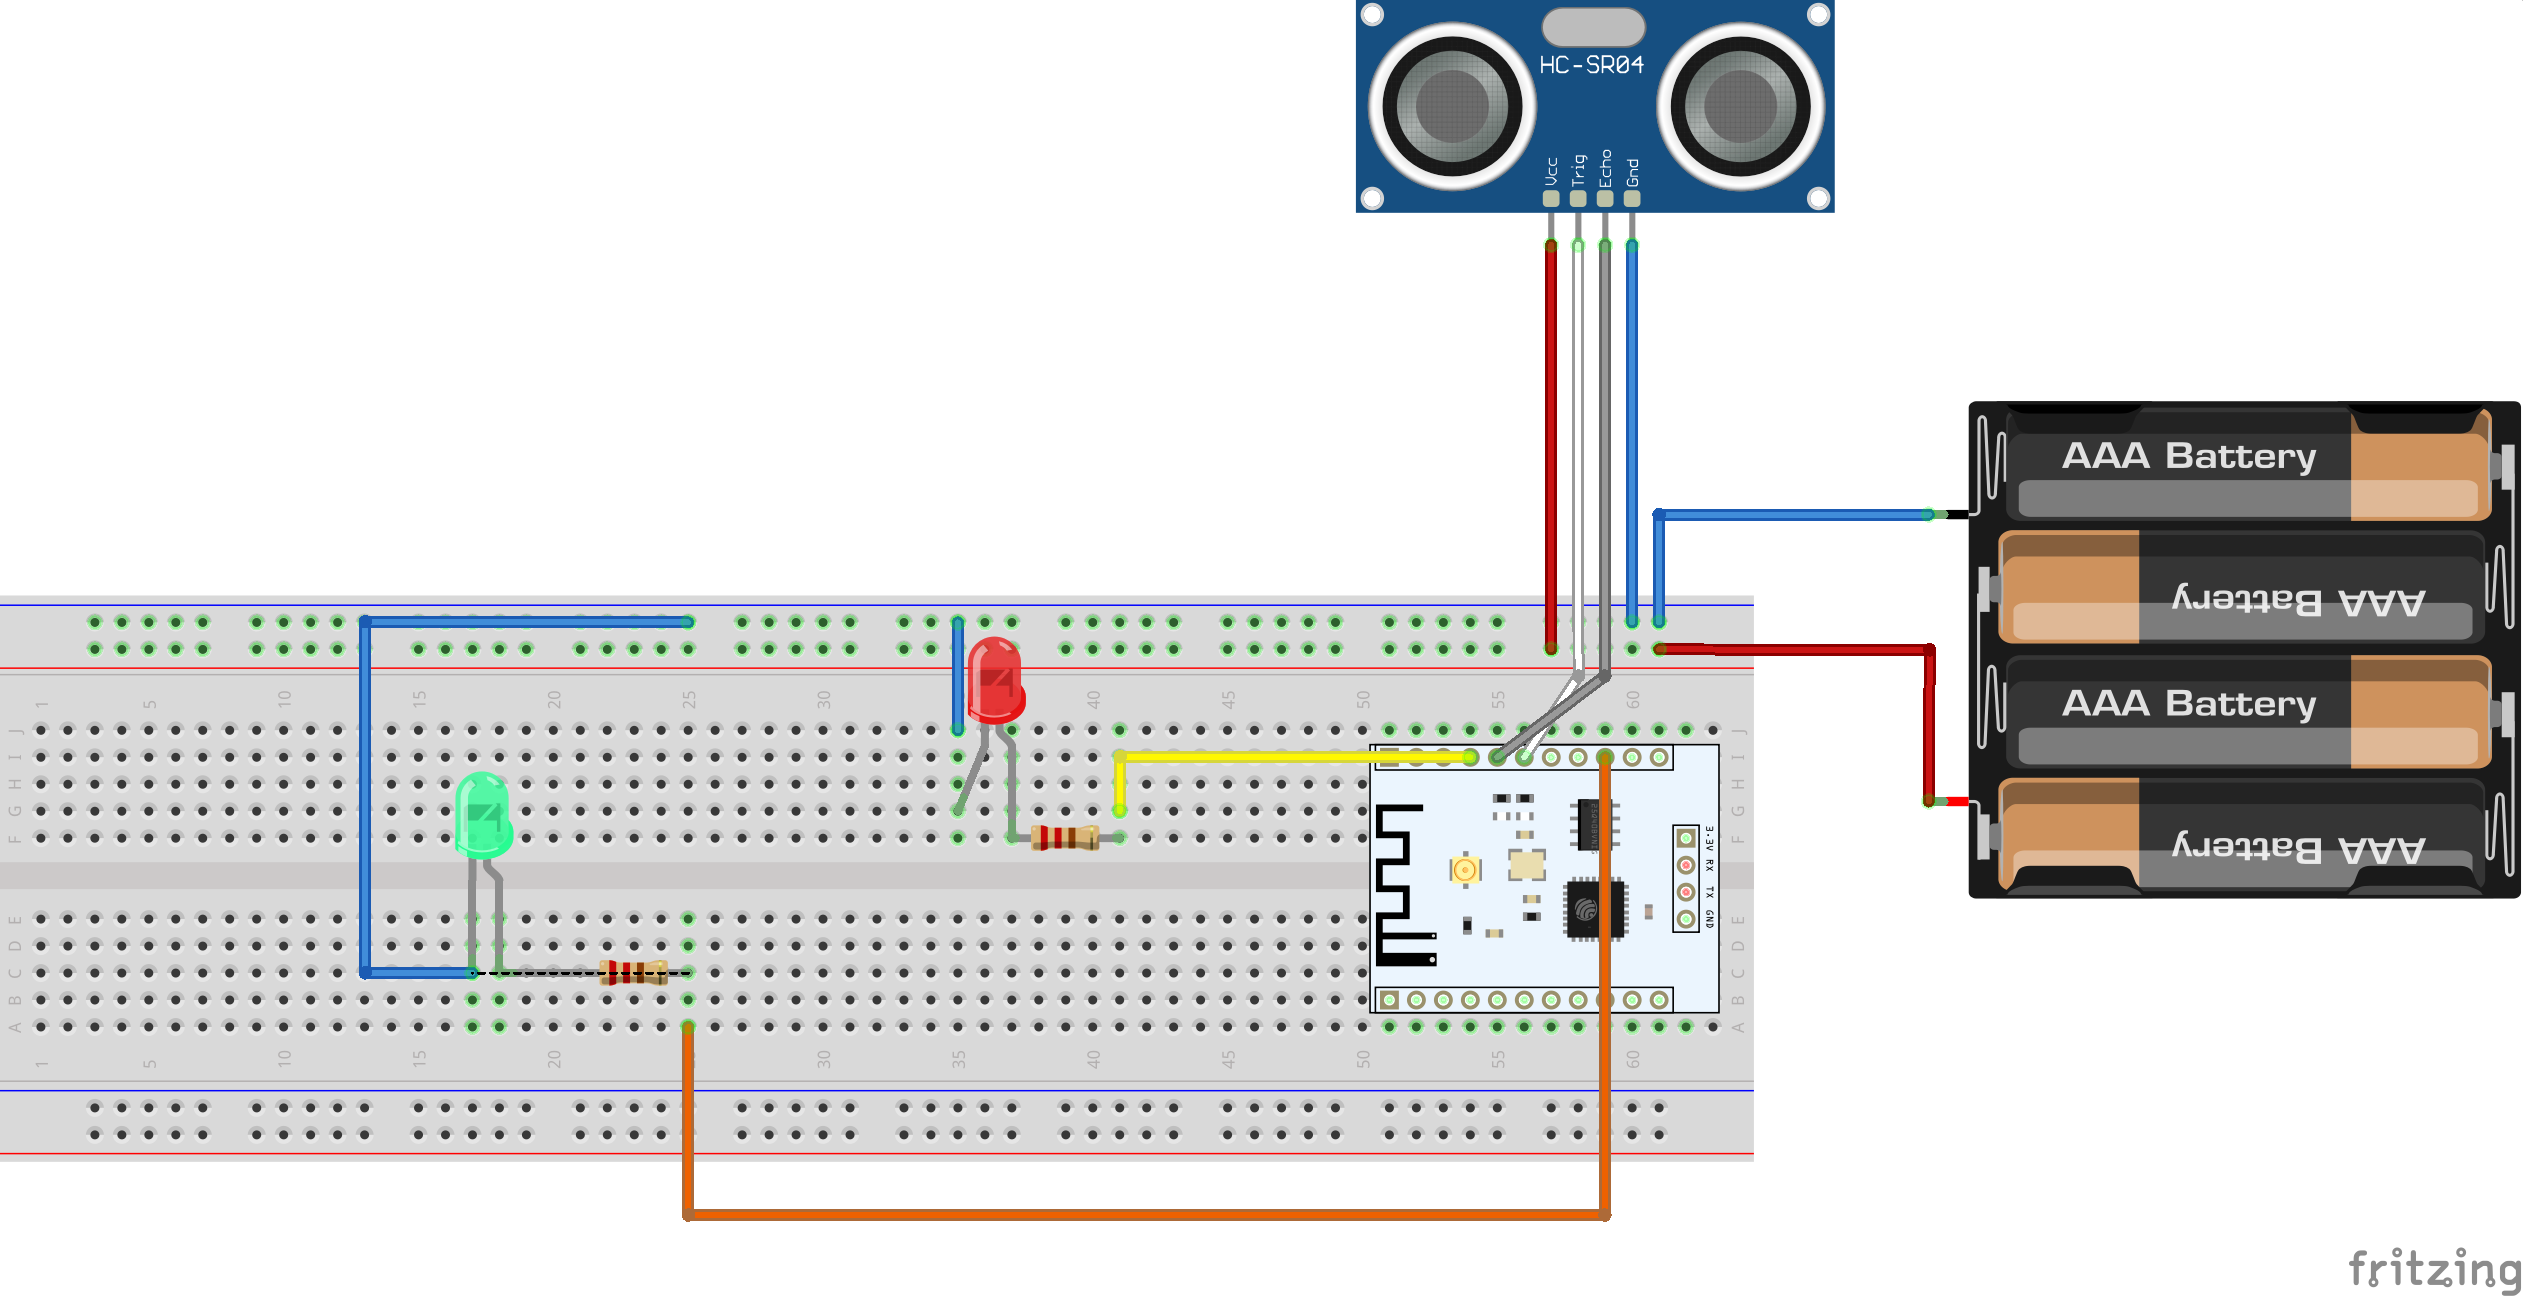
\includegraphics[scale=0.5]{pic/schema_bb.png}
\caption{Circuit of the system}
\label{schema_bb}
\end{figure}
\end{frame}

\begin{frame}{Micro controller program}
  Communication with the ultrasonic sensor
  \begin{itemize}
  \item implemented in the \texttt{loop()} function
  \item sensor is triggered with \texttt{digitalWrite(trigPin, LOW)} and
    \texttt{digitalWrite(trigPin, HIGH)}
  \item then the value is read with \texttt{pulseIn(echoPin, HIGH)} and the distance
    calculated basing on the time passed
  \end{itemize}
  Communication with the base station
  \begin{itemize}
    \item implemented in the \texttt{callback()} function, which overrides the
      one in Arduino libraries
    \item the \texttt{JSON} with thresholds information is received and parsed
    \item \texttt{LED}s are switched on/off accordingly
  \end{itemize}
\end{frame}


\begin{frame}{Node-Red Flow}
\begin{figure}
\hspace*{-0.6cm}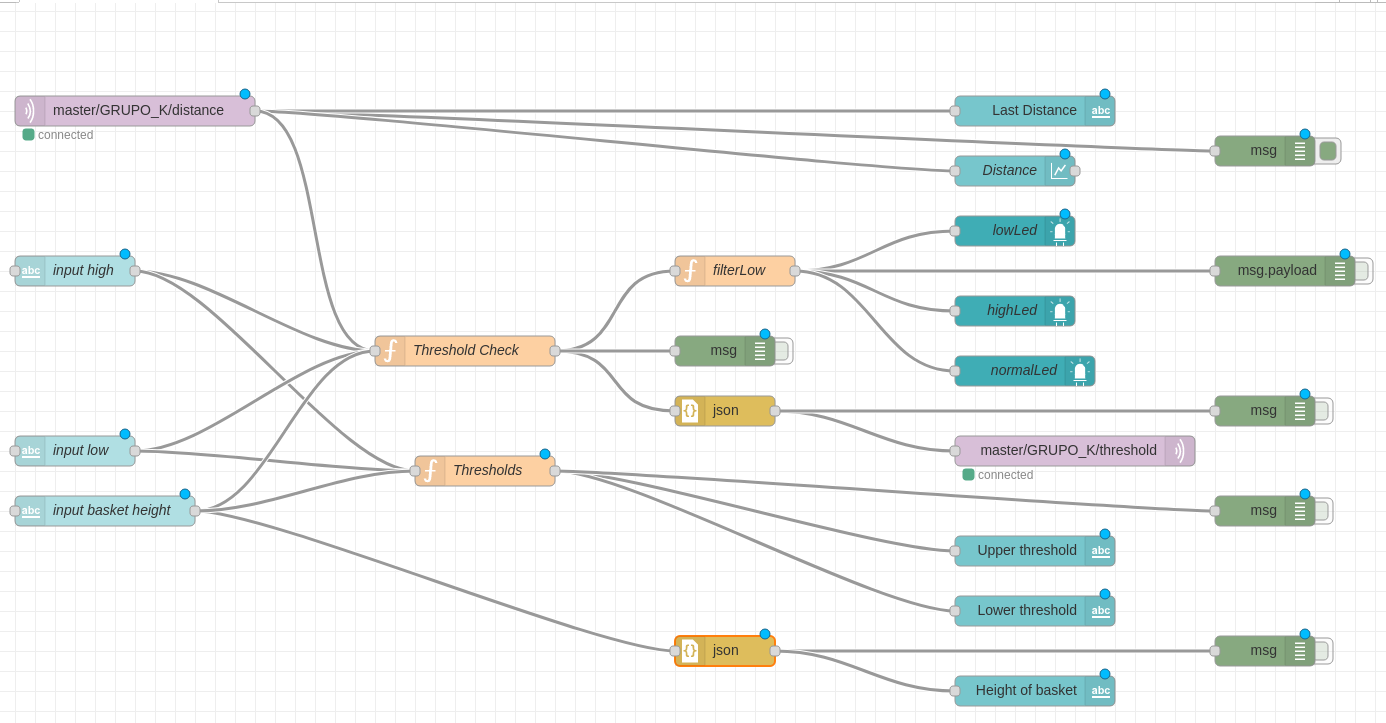
\includegraphics[scale=1.1]{pic/flowScheme.png}
\caption{Node-Red flow}
\label{flow}
\end{figure}
\end{frame}

\begin{frame}{Limitations}
\begin{itemize}
\item measurement fluctuations of the sensor $\to$ not reasonable values have to be filtered
\item needs constant Wifi connection between central computer and ESP to recognize thresholds
\item energy consumption scales with frequency of measurements
\item Battery should be changed/charged periodically
\end{itemize}
\end{frame}

\begin{frame}{}
\center
\huge{Thanks for your attention!}
\end{frame}

\end{document}